%!TEX root=report.tex
\subsection{Interpretation of PCA}

For each principal component (PC) one can compute its importance, its eigenvector (the loadings) in time as well as a spatial loading. 
\\
The most principal component PC\_1 has the following plots

\begin{figure}[H]
\centering
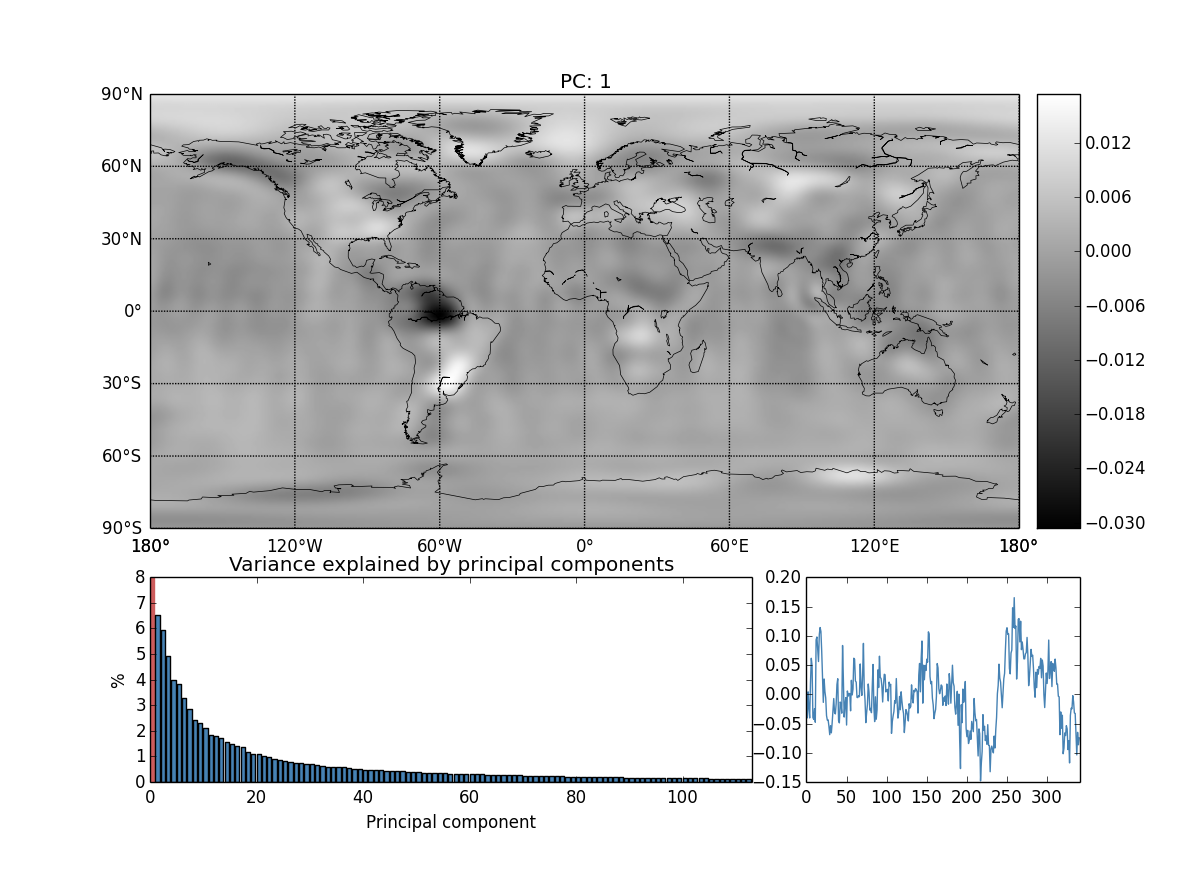
\includegraphics[width=1.0\linewidth]{figures/pc_1.png}
\end{figure}
From the spatial loading it seems that PC\_1 is designated, primarily, to account for the rain season in South America. 

\begin{figure}[H]
\centering
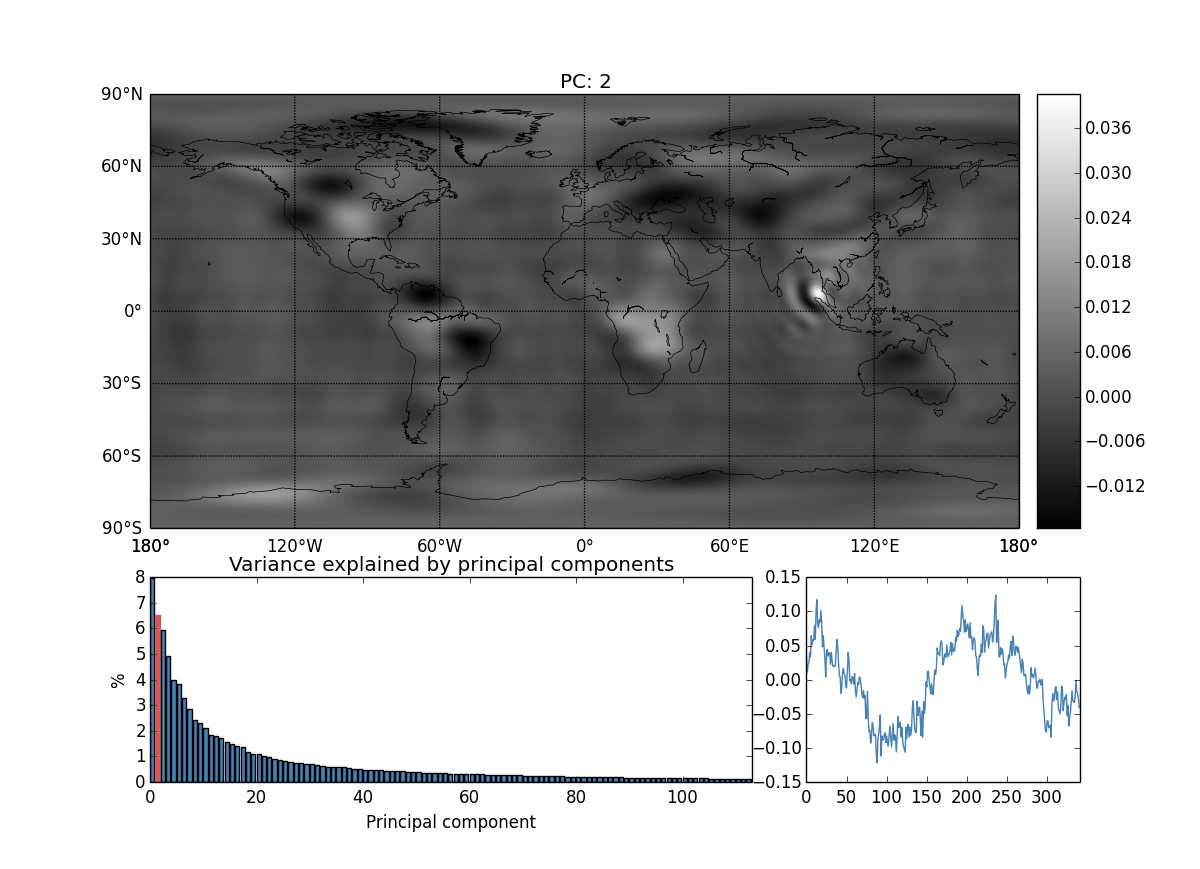
\includegraphics[width=1.0\linewidth]{figures/pc_2.png}
\end{figure}
PC\_2 seems more interesting than PC\_1. Right off the bat one notices the ripple effects with origin at the coast of Thailand which is due to the earthquake and following devastating tsunami which hit on the 26th December 2004. Secondly, PC\_2 also has significant loadings in South America, as well as spread out areas all over the globe. It also appears slightly peculiar that when looking at time dimension there seems to be wave like behavior although it is hard to tell exactly what this means.
